
En este capítulo se definirán los conceptos  o fundamentos de instrumentación estructural, sensores inteligentes y adquisición de datos, necesarios para llevar a cabo esta investigación.

\section{Estructuras civiles}

\subsection{Características generales}

Una estructura se refiere a un sistema de partes o elementos que se interconectan para cumplir una función es específico. En el caso de la ingeniería civil, suelen ser miembros que se utilizan para soportar una carga. Algunos ejemplos importantes son los edificios, los puentes y las torres; y en otras ramas de la ingeniería, son importantes las corazas de barcos y aviones, los sistemas mecánicos y las estructuras que soportan las líneas de transmisión eléctrica \citep{hibbeler1997structural}.

\subsection{Tipos de estructuras}

Según \citet{hibbeler1997structural}, cada sistema está formado por uno o varios de los cuatro tipos básicos de estructuras: 

\begin{itemize}
    \item Celosías.
    \item Cables y arcos.
    \item Armazones.
    \item Estructuras de superficie.
\end{itemize}

En general, estos elementos suelen soportar cargas, pueden ser estacionarios y también estar restringidos. Sus diferencias suelen basarse en la cantidad de fuerzas a las que están sujetos estos elementos en un instante dado.

La combinación de estos elementos y los materiales que los componen es lo que se denomina un sistema estructural. Estos sistemas, aunque sean pasados por alto, son utilizados diariamente por industrias y personas, siendo elementos claves en el desarrollo y progreso de la civilización actual.

\subsection{Comportamiento de las estructuras civiles}
\label{sec:comportamiento_estructuras}

La gran mayoría de los sistemas cuentan con una respuesta dinámica y estática. Ambas respuestas permiten conocer el comportamiento completo del sistema en estudio ante distintas entradas o en diferentes situaciones. Al estudiar el comportamiento estructural se encuentra una extensa literatura tanto para el estudio dinámico como para el régimen estático, recopilándose lo siguiente:

\begin{itemize}
    \item{Respuesta estática}: En la ingeniería civil toda estructura se diseña para que se encuentre en reposo cuando actúan sobre esta fuerzas externas, es decir, la estructura en conjunto debe cumplir con las condiciones de equilibrio, siendo la fuerza y el momento resultante sobre esta igual a cero en todo momento. Para describir estas condiciones de equilibrio se cuentan con herramientas matemáticas que proporcionan las condiciones necesarias para su cumplimiento. Estas ecuaciones permiten la resolución estática de la estructura, la cual permite determinar el valor de todas las incógnitas estáticas de interés \citep{basset2014analisis}.
    
    \indent Cuando las fuerzas que actúan sobre la estructura pueden calcularse a partir de las ecuaciones de equilibrio, se tiene una estructura en equilibrio y se denomina estructura estáticamente determinada. En caso de tenerse más fuerzas desconocidas que ecuaciones de equilibrio se habla de una estructura estáticamente indeterminada.

        \begin{itemize}
            \item Rigidez: Uno de los parámetros más importantes dentro de la respuesta estática es la rigidez. Esta se define como la propiedad que tiene un elemento estructural de soportar la deformación o deflección al estar bajo la acción de una fuerza o carga. Una medida de la rigidez viene dada por el Módulo de Young; esta es una constante del material y es independiente de la cantidad de material.
        \end{itemize}

    \item{Respuesta dinámica}: La dinámica estructural se encarga de estudiar el efecto que tienen cargas dinámicas sobre el sistema. La respuesta ante estos eventos, como pueden ser sismos, vientos, equipos mecánicos, paso de vehículos o personas, se denomina respuesta dinámica \citep{hurtado2000}. Además, la respuesta dinámica permite caracterizar algunos parámetros de gran interés para estudiar su comportamiento conocidos como parámetros modales. Estos parámetros surgen al estudiar las ecuaciones diferenciales que describen el movimiento de la estructura, partiendo de un modelo idealizado simple de masa concentrada como el de la Figura \ref{fig:masa_estructural}.
    
    \begin{figure}[H]
        \centering
        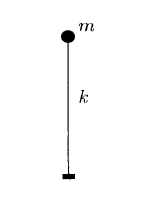
\includegraphics[width = 0.25\textwidth]{imagenes/cap1_marcoteo/modelo_masa_simple.png}
        \caption{Modelo de masa concentrada de 1 grado de libertad \citep{hurtado2000}.}
        \label{fig:masa_estructural}
    \end{figure}

    La dinámica de este modelo puede describirse utilizando la ecuación diferencial de movimiento:

    \begin{equation} \label{eq:vib_lib}
        m\ddot{u} + f_R(t) = p(t)
    \end{equation}

    La ecuación \ref{eq:vib_lib} se conoce como ecuación de vibración libre sin amortiguamiento. Donde $p(t)$ representa las cargas dinámicas y $f_R(t)$ la fuerza de restitución propia de un material elástico.  Esta ecuación es una ecuación diferencial de coeficientes constantes, que consta de una solución homogénea más una solución particular. La solución homogénea será la respuesta de la estructura a la vibración libre, es decir, si la masa de la Figura \ref{fig:masa_estructural} se deja oscilar libremente.

    Se sabe que una ecuación de este tipo tendrá una solución como:

    \begin{equation} \label{eq:sol_equ_dif}
        u = A.sin\omega t + B.cos\omega t
    \end{equation}

    La ecuación \ref{eq:sol_equ_dif} contiene información relevante para la caracterización dinámica de la estructura. Esta caracterización parte del estudio de los parámetros modales de la misma.

    Entre estos parámetros modales se encuentran: 
        \begin{itemize}
            \item Frecuencia natural: Toda estructura física tiene asociada una frecuencia de vibración natural. Las máquinas, los puentes, los edificios; todas estas estructuras vibran u oscilan al ser perturbadas o removidas de su estado de reposo inicial. Es una propiedad intrínseca del sistema y depende de su masa, rigidez y amortiguamiento. Todas tienen al menos una frecuencia natural y es posible que tengan múltiples frecuencias de resonancia \citep{irvine2000introduction}. 
            
                Se suele calcular la frecuencia natural de resonancia de un sistema libre usando:

                \begin{equation}
                    f =  \frac{1}{\sqrt{\frac{k}{m}}}
                \end{equation}

            \item Amortiguamiento: Toda estructura comienza a oscilar una vez es removida de su estado de reposo o equilibrio, sin embargo, ese movimiento no es perpetuo. El amortiguamiento se define como la capacidad de disipación de energía que posee la estructura bajo excitaciones externas. Al añadir el amortiguamiento de tipo viscoso, las soluciones a la ecuación \ref{eq:vib_lib} arrojan 3 posibles casos:
                \begin{enumerate}
                    \item Sistema críticamente amortiguado: El sistema no vibra.
                    \item Subamortiguado o amortiguado subcrítico: Caso más común por la naturaleza de los materiales utilizados en las estructuras. La respuesta del sistema decae con el tiempo de forma exponencial, como se puede ver en la Figura \ref{fig:resp_subamorti}. 
                    
                    \begin{figure}[H]
                        \centering
                        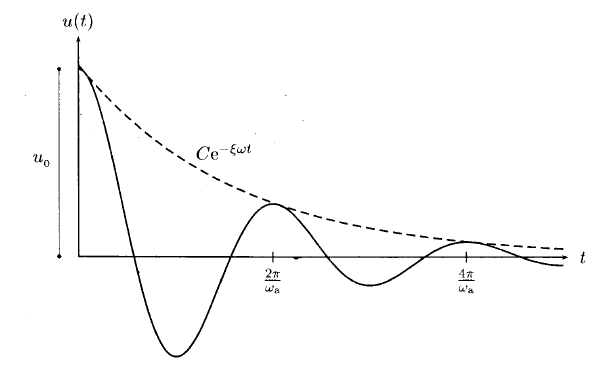
\includegraphics[width = 0.7\textwidth]{imagenes/cap1_marcoteo/respuesta_sist_subamorti.png}
                        \caption{Respuesta ante vibración libre en sistema Subamortiguado \citep{hurtado2000}.}
                        \label{fig:resp_subamorti}
                    \end{figure}

                    \item Sobreamortiguado: Nunca se encuentra esta respuesta en sistemas estructurales por los materiales utilizados.
                \end{enumerate}
            
        \end{itemize}        
\end{itemize}

% \subsection{Respuesta en frecuencia}

%     Incluir?

\subsection{Daño en estructuras}

El daño a una estructura civil o mecánica puede definirse como todo cambio en las propiedades materiales o geométricas del material que llegan a afectar de forma adversa la confiabilidad y el desempeño actual o futuro del sistema. Por tanto, el daño es una comparación entre el sistema en cuestión en 2 instantes de tiempo distintos \citep{farrar2007introduction}. Estos efectos adversos pueden ser, en el caso estructural, desplazamientos, estrés indeseado en un elemento o vibraciones estructurales indeseadas \citep{chen2018}.

Todas las estructuras civiles, como puentes y edificios, acumulan daño de forma continua a medida que están en servicio y transcurre su vida útil. Este daño puede manifestarse como fracturas, fatiga, socavaciones o desprendimiento del concreto. El daño que no sea detectado puede conducir a una falla estructural que a su vez ocasione pérdidas humanas. Por tanto, es imperativo y necesario detectar el daño en una estrcutrura tan pronto como sea posible, \citep{chen2018}.

Entre algunos de los factores que influyen del deterioro de una estructura se encuentran:
    
        \begin{itemize}
            \item Proceso de degradación natural de los materiales.
            \item Corrosión del acero de refuerzo.
            \item Evento sísmico, incendios o condiciones de guerra.
            \item Carga por encima del límite de diseño.
        \end{itemize}
    
Las escalas de tiempo y de extensión del daño son diversas. Por ejemplo, el deterioro por el paso del tiempo bajo ciertas condiciones climáticas es muy lento comparado al daño causado por un evento catastrófico.

\subsection{Principios de la Sismoresistencia}

Una edificación sismorresistente es aquella que está diseñada y construida para soportar las fuerzas causadas por eventos sísmicos. Sin embargo, incluso las edificaciones diseñadas y construidas según las normas sismorresistentes pueden sufrir daños en caso de un terremoto muy fuerte, sin embargo, las normas establecen los requisitos mínimos para proteger la vida de
las personas que ocupan la edificación

Algunas de las características de una estructura sismoresistente son:

        \begin{itemize}
            \item Forma regular.
            \item Bajo peso.
            \item Mayor rigidez.
            \item Buena estabilidad.
            \item Suelo firme y buena cimentación.
            \item Materiales competentes.
            \item Capacidad de disipación de energía.
            \item Fijación de acabados e instalaciones.
        \end{itemize}

En Venezuela las estructuras deben cumplir con la Norma Venezolana COVENIN 1756-1:20019 (Construcciones Sismorresistentes), \citep{covenin}.

Se ha observado que al estudiar el comportamiento de las estructuras luego de un evento sísmico, es evidente que cuando se toman en cuenta las normas de diseño sismorresistente dispuestas en la ley y la construcción es debidamente supervisada, los daños estructurales resultan ser considerablemente menores que en las edificaciones en las cuales no se cumplen los requerimientos mínimos indispensables estipulados en la norma, \citep{blanco2012criterios}.

\subsubsection{Importancia de la instrumentación} La instrumentación estructural permite medir y monitorear las acciones y respuestas estructurales ante distintos eventos. Esto proporciona datos en tiempo real y fuera de línea sobre el comportamiento dinámico y estático de la estructura, como deformaciones, aceleraciones y desplazamientos, que son fundamentales para evaluar y verificar si la estructura cumple con los criterios de diseño sismoresistente establecidos en la norma.

La instrumentación estructural ayuda a validar los modelos y suposiciones utilizados en el diseño estructural inicial. Al comparar los datos recopilados por la instrumentación durante un evento sísimco con las predicciones del modelo, es posible verificar si la estructura se comporta de acuerdo con las expectativas y si cumple con los criterios de seguridad establecidos en la norma.

Además, el monitoreo continuo de la estructura permite conocer el estado actual de la misma, tema que representa la idea principal del Monitoreo de Salud Estructural, permitiendo a los ingenieros evaluar si se sigue cumpliendo con la norma para luego tomar decisiones y actuar en pro de la seguridad de la edificación.


\section{Salud estructural}

\subsection{Definición}


El proceso de implementar una estrategia de identificación de daño para estructuras civiles, mecánicas o aeroespaciales se conoce como Monitoreo de Salud Estructural (SHM por sus siglas en inglés). Esta estrategia requiere medir las condiciones y el ambiente en el que opera la estructura, además de la respuesta de la misma durante un período de tiempo tomando muestras periódicamente espaciadas, \citep{farrar2007introduction}.


La estrategia del SHM requiere de equipos multidisciplinarios de ingeniería, ya que necesita de una red de sensores que midan las variables de interés, el procesamiento y análisis de los datos obtenidos y posteriormente una prognosis del daño para una eventual toma de decisiones. El objetivo del SHM es proveer, en toda la vida útil de la estructura, un diagnóstico del estado de sus materiales constitutivos, de los diferentes elementos que la componen y de la estructura en sí como el conjunto de todas estas partes. Esto para garantizar que la misma se comporte dentro de los parámetros iniciales de diseño, aunque estos cambien por la acción natural del tiempo, el ambiente y accidentes, \citep{balageas2010structural}.

El resultado de este proceso es información actualizada sobre el estado de la estructura y sobre su capacidad actual para seguir desempeñado la función para la cual fue diseñada.

Según \citet{enckell2006structural}, el SHM se ha convertido en una herramienta muy conocida y utilizada en ingeniería estructural en los últimos años en diferentes países.

\subsection{Reseña histórica}

Las técnicas de detección de daño basadas en vibración tienen sus primeras aplicaciones desde hace cientos de años. En la antigüedad, los constructores golpeaban las estructuras para encontrar espacios vacíos o grietas en elementos de arcilla. La utilidad de estas inspecciones tan simples indicaban que la sofisticación de estos métodos podía proveer información muy valiosa sobre el elemento de interés, sin embargo, esto requiere de instrumentos y herramientas matemáticas que se han desarrollado con el pasar de los años. El auge en el uso de SHM en años recientes es consecuencia de la evolución y miniaturización del hardware computacional actual.


El uso más exitoso del SHM ha sido el monitoreo de la condición de máquinas rotativas, las cuales actualmente han adoptado un enfoque de indetificación de daño sin basarse en un modelo de forma casi exclusiva, \citep{farrar2007introduction}.

En los años 70 la industria petrolera consideró el uso de técnicas basadas en vibración para identificar daños en plataformas costa-afuera, este enfoque se diferenció de las máquinas rotativas al estudiar un sistema en donde la ubicación del daño es desconocida y difícil de instrumentar.

En esa misma época, la comunidad aeroespacial y la \textit{National Eeronautics Space Agency} (NASA), comenzaron a estudiar esta técnica de identificación de daño en los comienzos de la era de lanzamientos espaciales. Este trabajo continúa hoy en día y el \textit{Shuttle Modal Inspection System} (SMIS) se desarrolló para identificar fatiga en distintos componentes de cohetes espaciales reusables, los cuales representan el futuro de esta industria.


Usualmente, los enfoques de estas industrias se basan en comparar modelos analíticos de estructuras sin daño con las mediciones de estructuras con daño, observando principalmente las propiedades modales de las mismas. Se ha observado que cambios en la rigidez en ambos modelos han permitido localizar y cuantificar el daño, \citep{farrar2007introduction}.

Inicialmente, las técnicas no destructivas fueron introducidas en la ingeniería civil a mediados de los años 40, \citep{mohamed2014}. La necesidad principal surgió en determinar propiedades del concreto fresco \textit{in-situ}. Estas técnicas, que buscaban evaluar la homogeneidad y la resistencia del concreto eran en su mayoría pruebas con martillo y pruebas de \textit{pull-out}. A medida que las estructuras envejecieron, los ingenieros necesitaban idear maneras de medir o estimar las propiedades mecánicas de los elementos que consituyen las estructuras, además de detectar daños que no eran fáciles de observar por la envergadura de las estructuras civiles que se han desarrollado en los últimos 150 años. Es ahí, en los años 70, donde surgen nuevas estrategias no destructivas tales como:

    \begin{itemize}
        \item Emisión acústica.
        \item Métodos de ultrasonido y radar.
        \item Termografía.
        \item Métodos basados en vibración
    \end{itemize}

La comunidad de ingeniería civil ha estudiado la identificación de daño basada en vibración en puentes y edificios desde comienzos de los años 80. Las propiedades modales han sido estudiadas por diferentes autores y son las principales características que se analizan al identificar daño. El auge del SHM es tal, que algunos países asiáticos han implementado regulaciones en donde las compañías constructoras deben verificar la salud estructural de los puentes periódicamente. Estas regulaciones han provocado que la investigación e inversión en esta área siga aumentando de forma considerable \citep{chen2018}. 

\subsection{Línea de trabajo del Monitoreo de Salud Estructural}

Los sistemas de SHM consisten de varios elementos que permiten a los ingenieros tener información sobre el estado de una estructura, entre esos elementos se encuentran:

\begin{itemize}
    \item Sensores.
    \item Sistemas de adquisición de datos.
    \item Sistema de transmisión de datos.
    \item Sistema de procesamiento de datos.
    \item Sistema de manejo y almacenamiento de datos.
    \item Equipo de análisis y toma de decisiones.
\end{itemize}

\begin{figure}[H]
    \centering
    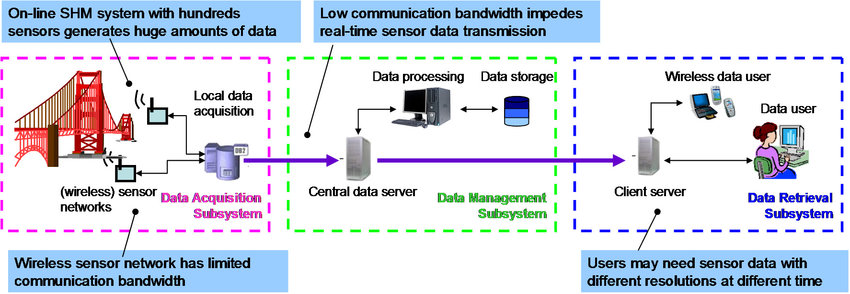
\includegraphics[width = 0.9\textwidth]{imagenes/cap1_marcoteo/Schematics-of-an-on-line-structural-health-monitoring-system-and-technical-challenges.png}
    \caption{Esquema de un sistema de SHM \citep{lijianfoto2015}.}
    \label{fig:esquema_gral_SHM}
\end{figure}


Autores como \citet{rytter1993vibration} y \citet{farrar2007introduction} han esquematizado la estrategia del SHM categorizando el daño en una estructura por niveles de la siguiente forma:

\begin{enumerate}
    \item Nivel I (detección del daño) ¿Presenta daño el sistema? Es una indicación cualitativa de que puede haber daño presente en la estructura.
    \item Nivel II (localización o ubicación del daño) ¿Dónde está presente el daño? Indica la posible localización del mismo. 
    \item Nivel III (clasificación del daño) ¿Qué tipo de daño está presente? Da información sobre el tipo de daño.
    \item Nivel IV (alcance/grado/extensión del daño) ¿Cuál es el alcance del daño? ¿Qué tan grave es? Da un estimado del alcance.
    \item Nivel V (prognosis del daño) ¿Cuánta vida útil le queda a la estructura? Da un estimado de la seguridad de la estructura.
\end{enumerate}

En la mayoría de los casos, para alcanzar el nivel final es necesario obtener información sobre los niveles previos. Esto indica que a medida que se sube de nivel se tiene un mayor conocimiento sobre el estado de la estructura.

De acuerdo a \citet{chen2018}, los primeros dos niveles, detección y localización, generalmente pueden alcanzarse usando métodos de detección basados en vibración para obtener mediciones sobre la respuesta dinámica de la estructura.

Por su parte, \citet{chen2018} describe el proceso de SHM en general como:

\begin{enumerate}
    \item Observación.
    \item Evaluación.
    \item Calificación.
    \item Gestión.
\end{enumerate}

La estrategia de Monitoreo de Salud Estructural podría resumirse en el siguiente diagrama:

\begin{figure}[H]
    \centering
    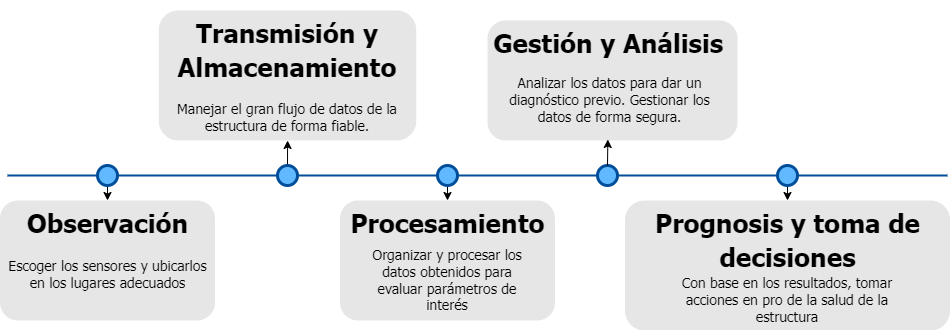
\includegraphics[width = \textwidth]{imagenes/cap1_marcoteo/Diagrama SHM timeline.png}
    \caption{Diagrama general del proceso de SHM.}
    \label{fig:diag_SHM}
\end{figure}

\subsection{Criterios de evaluación}

Como se definió anteriormente, el daño estructural puede tener distintas causas y formas. Lo que se sabe con certeza es que una estructura, una vez entra en funcionamiento, análogo a los seres humanos al nacer, estará sujeta a envejecimiento natural y a condiciones adversas. Ahora bien, en el caso del SHM, surge la siguiente pregunta: ¿Qué se debe medir para poder detectar este daño?. 

Numerosos autores concluyen que uno de los indicativos de daño de una estructura viene dado por los parámetros modales definidos anteriormente, frecuencia y amortiguamiento. Esta relación entre los parámetros modales y el daño viene dada por la premisa de que todo daño presente en la estructura se reflejará en un cambio en las propiedades dinámicas de la misma. \citet{worden2009modal}, comprobó la relación entre el cambio progresivo en todas las frecuencias naturales de 15 vigas estudiadas a las cuales se les introdujo un daño relacionado con un cambio del Módulo de Young, el cual, como fue mencionado anteriormente, provee un indicativo de la rigidez de un elemento.

Anterioremente en la ecuación \ref{eq:vib_lib} se definió un sistema con un grado de libertad (DOF por sus siglas en inglés), sin embargo, en la realidad las estructuras tienen múltiples grados de libertad, por lo que es conveniente modelarlas de estar forma para obtener resultados más precisos. En el caso de los sistemas con ``n grados de libertad'', la ecuación de movimiento que describe la dinámica del sistema en vibración libre vendrá dada por:

\begin{equation} \label{eq:ecu_movimiento}
    M\ddot{u} + C\dot{u} + Ku = 0
\end{equation}

Donde M, C y K representan las matrices de masa, amortiguamiento y rigidez de la estructura, respectivamente.

Si se asume un sistema sin amortiguamiento, a fines de estudiar el efecto que tiene sobre la rigidez un cambio en los parámetros modales,  de la ecuación \ref{eq:ecu_movimiento} se obtiene: 

\begin{equation} \label{eq:ecu_movimiento_sindamp}
    M\ddot{u} + Ku = 0
\end{equation}

Si se asume una solución oscilatoria pura, por ser un sistema sin amortiguamiento:

\begin{equation} \label{eq:sol_ecu_motion}
    u = ve^{jwt}
\end{equation}

Al derivar, sustituir y despejar en la ecuación \ref{eq:ecu_movimiento_sindamp} se obtiene:

\begin{equation} \label{eq:eig_problem}
    (K - \lambda M)\phi = 0
\end{equation}

Esta ecuación \ref{eq:eig_problem} representa claramente un problema de autovalores, donde $\lambda$ representa los autovalores asociados a las frecuencias naturales del sistema y $\phi$ representa el autovector de desplazamiento.

Si se introduce un pequeño cambio $\Delta K$ con perturbaciones similares en los otros parámetros:

\begin{equation}
    [(K - \Delta K) - (\lambda - \Delta\lambda)(M - \Delta M)](\phi - \Delta\phi) = 0
\end{equation}

El daño estructural suele venir asociado a un cambio en la rigidez, más no a cambios en la masa de la estructura, por lo que se asume $\Delta M = 0$, \citep{hearn1991modal}. A su vez, se tiene que $(K - \lambda M)\phi = 0$. \citet{mohamed2014}, \citet{shi1998structural} y \citet{hearn1991modal} desarrollan estas ecuaciones obteniendo la siguiente relación:

\begin{equation} \label{eq:relacion_final}
    \Delta\lambda = \phi^T \Delta K \phi
\end{equation}

De la ecuación \ref{eq:relacion_final} se observa que cambios en los autovalores $\lambda$ que representan las frecuencias naturales, y en los autovectores $\phi$ (formas modales) están directamente relacionados con cambios en la matriz de rigidez (K) del sistema. De aquí surge el interés en monitorear los parámetros modales como indicadores de daño estructural. Es importante recalcar que estos cambios son indicativos de daño global, más no de la localización del mismo, para lo que se necesitan otras técnicas, \citep{mohamed2014}.

\subsection{Variables de interés}

Tomando en cuenta la relación entre los parámetros modales y el daño presente en una estructura, es preciso definir las variables de interés para el monitoreo de la salud estructural de una estructura. Si bien existen distintas varibales que permiten obtener información valiosa sobre la estructura en estudio, algunas de estas no proporcionan información global del daño, como es el caso de las formas modales y la deflección local \citep{rytter1993vibration}. Sin embargo, estas mediciones proveen indicativos de la ubicación del daño, por lo que pueden constituir parte del sistema de monitoreo en una etapa más avanzada, es decir, una vez el daño fue detectado. A continuación se presentan las más relevantes para el daño global:

    \begin{itemize}
        \item Frecuencias naturales y amortiguamiento: Los parametros modales de la estructura están ligados de forma directa al estado de la misma. El deterioro en una edificiación induce cambios en la rigidez estructural, como se observa claramente en la ecuación \ref{eq:relacion_final}. El daño puede tener efectos distintos en cada modo o cada frecuencia de vibración, por lo que es importante no ubicar los sensores sobre los nodos modales, ya que experimentos han demostrado la ineficacia en las mediciones. Usualmente, el daño se refleja como una disminución en las frecuencias naturales afectadas, aunque se han observado casos de aumento en las frecuencias de vibración en estructuras de concreto pretensado, \citep{rytter1993vibration}.
        
        A su vez, el amortiguamiento varía al introducir daño en la estructura, puesto que su capacidad de disipar energía se ve afectada. Usualmente, los investigadores observan un aumento en el amortiguamiento a medida que el daño aumenta, como se ha demostrado experimentalmente por autores como \citet{hearn1991modal} y \citet{rytter1993vibration}.

        \item Temperatura y humedad: En los sistemas de monitoreo, la detección del daño estructural puede tomar períodos de tiempo considerables, durante los cuales las características sujetas a temperatura y humedad, sufren cambios que afectan la respuesta estructural.
                
        Es evidente que las condiciones climáticas contribuyen con el deterioro de las edificaciones. A pesar de esta conclusión, relacionar las condiciones climáticas con el daño introducido usando mediciones ambientales es difícil. La medición de estas variables suele tomarse en cuenta para poder cuantificar el cambio que producen estas condiciones en los demás indicadores de daño. \citet{rytter1993vibration} observó que la humedad y temperatura afectaban las mediciones de amortiguamiento. Por su parte, \citet{mohamed2014}, observó que las frecuencias naturales de barras y vigas disminuían a medida que aumentaba la temperatura. A su vez, \citet{sohn2007effects} determinó que cuando hay humedad presente en el ambiente, los puentes de hormigón absorben una cantidad considerable de esta, lo que aumenta sus masas y altera sus frecuencias naturales.
        
        \item Inclinación y desplazamiento: Una de las variables más comunes en Sistemas de Monitoreo de Salud Estructural es el desplazamiento lineal, que refleja de forma directa el comportamiento de un elemento o estructura. Esta podría considerarse una variable de tipo estático, ya que a pesar de variar con el tiempo, es decir, depender de un componente dinámico como el viento o la carga vehicular, su interacción con el medio suele ser quasi-estática, causada por la carga estática de la estructura, efectos térmicos y asentamiento.
        
        Los inclinómetros son utilizados en elementos estructurales para medir el desplazamiento lineal de un elemento respecto a una referencia. Suelen ser utilizados para dar una idea de la fijación que presentan los puentes en sus soportes o para monitorear a largo plazo el movimiento de estructuras sobre superficies propensas a deslizamientos.

        La deflección, que puede medirse haciendo uso de inclinómetros los cuales han generado un gran interés en la industria por su sensibilidad y bajo costo, es una variable muy importante a medirse en una estructura. La deflección puede ser consecuencia de la corrosión de los elementos de soporte, pérdida del pretensado o el crecimiento de grietas en el concreto. Es decir, a medida que la deflección aumenta se acelera la acumulación de daño, por tanto, medir esta variable puede proveer alertas tempranas sobre posibles cambios estructurales o deterioro \citep{zhang2017bridge}.

        Autores como \citet{komarizadehasl2022development} destacan la medición de la inclinación en las últimas décadas en el sector de la Ingeniería Estructural, inicialmente con propósitos geotécnicos. Sin embargo, gracias a los avances tecnológicos en los sensores, se comenzó a emplear su uso en otras áres, sobre todo en el monitoreo de salud estructural.

    \end{itemize}

\section{Métodos de identificación de daño}

    \subsection{Basado en modelo} El método basado en modelo consiste en estructurar un modelo de elemento finito que será utilizado para identificar y localizar el daño en la estrucutra. Su precisión dependerá de su nivel de correlación con la estructura real, por lo que este método suele emplearse luego de realizar mediciones sobre el sistema y obtener datos experimentales, que permiten ajustar el modelo y disminuir las discrepancias, \citep{garcia2023review}.

    \subsection{Basado en respuesta} El monitoreo de salud estructural basado en datos hace uso de datos reales de la estructura obtenidos a través de mediciones experimentales en sitio. Diferentes arreglos de sensores se utilizan para medir los parámetros de interés para el SHM \citep{mohamed2014}.

    En este método, se comparan los datos obtenidos con los datos históricos de la estructura sin daño. Esta información previa puede ser suministrada por un software de simulación de la estructura basado en sus características iniciales de construcción. Autores como \cite{fritzen2005vibration} estudiaron el uso de la información modal mediante estudios de vibración ambiental y forzada.

\section{Ensayos estructurales}

Los ensayos estructurales se utilizan para evaluar la integridad y el comportamiento de estructuras. Estos ensayos pueden clasificarse en invasivos y no invasivos, según la forma en que interactúan con la estructura en estudio. A continuación, se describen brevemente ambos tipos de ensayos:

\subsection{Ensayos invasivos}

\begin{itemize}
    \item{Extracción y análisis de núcleos de concreto:} Estos ensayos implican la extracción de muestras de material de la estructura para someterlas a pruebas en laboratorio. Por ejemplo, se pueden realizar pruebas de compresión, tracción o flexión en muestras de concreto, acero u otros materiales utilizados en la construcción. A su vez, los núcleos se someten a distintas condiciones de temperatura y humedad para evaluar su comportamiento.
    \item{Pruebas de carga:} Consisten en aplicar cargas controladas a la estructura y medir su respuesta. Esto puede incluir la aplicación de cargas estáticas o dinámicas para evaluar la capacidad de carga, la rigidez y la respuesta estructural.

\end{itemize}
   
\subsection{Ensayos no invasivos o mínimamente invasivos} 

Los ensayos no invasivos se introdujeron en la ingeniería civil durante los años 40 \citep{mohamed2014}. Desde entonces, muchas de estas pruebas han sido estandarizadas, siendo las normas COVENIN 2221:84 y COVENIN 318-84 algunas de las normativas para este tipo de ensayos en Venezuela. 

Con el envejecimiento progresivo de las estructuras, la industria de la construcción ideó nuevas técnicas durante los años 70, permitiendo evaluar de forma más rigurosa las propiedades mecánicas de los materiales y detectar anomalías o daños sin perjudicar la estructura. Algunos de estos métodos se describen a continuación:

\begin{itemize}
    \item{Inspección visual:} Estos ensayos se basan en la inspección visual de la estructura para detectar signos de daño, deformaciones o fallas.

    \item{Radiografía:}  Se utilizan rayos X o rayos gamma para inspeccionar estructuras en busca de defectos internos, como grietas, inclusiones de materiales o corrosión.

    \item{Ultrasonido:} Estos ensayos se basan en la inspección visual de la estructura para detectar signos de daño, deformaciones o fallas.

    \item{Análisis de vibración estructural:} Los ensayos de vibración permiten describir y evaluar el comportamiento dinámico de la estructura en estudio. Se hace uso de acelerómetros para obtener registros del movimiento estructural ante distintos tipos de vibración y posteriormente se ejecuta el estudio de estos datos en el dominio de la frecuencia, prestando especial interés a las frecuencias de resonancia presentes en el espectro, tanto propias del sistema (modos de vibración), como ajenas al mismo que puedan afectar su funcionamiento.
\end{itemize}


%MICROS


\section{Microcontroladores (MCU)}

\subsection{Definición y características}

Un microcontrolador es un dispositivo diseñado para controlar tareas específicas en sistemas electrónicos. Usualmente se fabrican utilizando técnicas de miniaturización como VLSI (\textit{Very Large Scale Integration}). Varios tipos de microcontroladores están disponibles en el mercado con diferentes características, clasificándose generalmente por su tamaño en bits (2, 4, 8, 64 y 128 bits). Los microcontroladores encapsulan en un solo chip un microprocesador, memoria, periféricos de entrada/salida y otros componentes necesarios para controlar y ejecutar tareas específicas. Esencialmente, es un pequeño ordenador en un solo circuito integrado.

Los microcontroladores se utilizan en una amplia variedad de aplicaciones donde se requiere control y procesamiento de datos en tiempo real. Pueden encontrarse en dispositivos electrónicos como electrodomésticos, automóviles, equipos médicos, sistemas de seguridad, robots, entre otros.

Entre los elementos que componen un microcontrolador se encuentran:

\begin{itemize}
    \item Unidad Central de Procesamiento.
    \item Memoria RAM (\textit{Random Access Memory}) y ROM (\textit{Read Only Memory}).
    \item Periféricos.
    \item Convertidores analógico-digital (ADC) y digital-analógico (DAC).
    \item Temporizadores.
    \item Interfaces de comunicación.
    \item Real Time Clock (RTC).
\end{itemize}

En la figura \ref{fig:ESP32_Block_Diagram} se observa el diagrama de bloques de las partes que constituyen un microcontrolador del fabricante Espressif.

\begin{figure}[H]
    \centering
    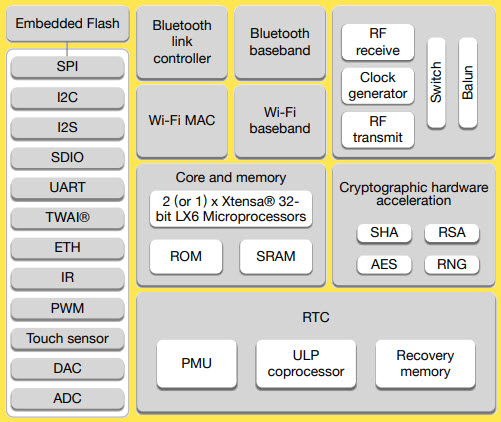
\includegraphics[width = \textwidth]{imagenes/cap1_marcoteo/ESP32-Block-Diagram.jpg}
    \caption{Esquema general del microcontrolador ESP32 (Espressif).}
    \label{fig:ESP32_Block_Diagram}
\end{figure}

\subsection{Placas de desarrollo}

Actualmente existen numerosas formas de hacer uso de las bondades que ofrecen los microcontroladores, especialmente al utilizar las distintas placas de desarrollo que se han diseñado para facilitar su programación e interfaz, ofreciendo la capacidad de comunicarse con un computador de forma sencilla a través del puerto USB, brindando distintas funcionalidades a los periféricos y facilitando la alimentación al microcontrolador. Estas tarjetas han logrado disminuir el costo del uso de los microcontroladores, especialmente para la creación de prototipos que permiten evaluar la factibilidad de un proyecto antes de diseñar la placa de circuito impreso (PCB por sus siglas en inglés) con un microcontrolador pre-programado.

Las placas de desarrollo se pueden sudividir en:


\begin{itemize}
    \item \textit{System-on-Chip} (SoC).
    \item Basadas en microcontrolador (\textit{MCU-based}).
    \item \textit{Single-Board-Computer} (SBC).
\end{itemize}
Algunas de los fabricantes de tarjetas de desarrollo más reconocidos que cuentan con comunidades y soporte técnico son:

\begin{itemize}
    \item STMicroelectronics.
    \item Espressif.
    \item Texas Instruments.
    \item Nordic Semiconductors.
    \item NXP.
    \item Arduino.
    \item Raspberry Pi.

\end{itemize}

\subsection{Protocolos de comunicación}

Los protocolos de comunicación fueron desarrollados y estandarizados para que sensores, drivers y diferentes periféricos y dispositivos de entrada y salida pudieran comunicarse entre sí sin problemas, evitando la tediosa tarea de buscar dispositivos compatibles dependiendo de la aplicación y el fabricante a utilizar. 

Cada protocolo tiene sus características y aplicaciones, siendo diseñados para propósitos distintos. El desarrollador o diseñador puede escoger uno o más dependiendo de las especificaciones del producto a diseñar. A continuación se mencionan los más utilizados por los microcontroladores:

\begin{itemize}
    \item UART (\textit{Universal Asynchronous Receiver-Transmitter}): Uno de los protocolos más simples y comúnmente utilizado para comunicación entre dos dispositivos. Como su nombre lo indica, no utiliza una señal de reloj para sincronizar al dispositivo transmisor y receptor. Es por esto que, a diferencia de la mayoría de los protocolos, solo utiliza 2 cables para lograr la comunicación.
    
    UART requiere de bits de inicio y parada para detectar datos entrante, además de requerir que la velocidad de comunicación sea configurada al mismo valor en bits por segundo (bps) en el receptor y transmisor. Admite comunicaciones Simplex, Half-Duplex y Full-Duplex.
 
    \item I2C (\textit{Inter-Integrated Communication}):  El protocolo I2C fue desarrollado por Philips Semiconductors en 1982. Se utiliza principalmente para comunicación entre periféricos, sensores y circuitos integrados en distancias cortas. Requiere 2 cables de datos (SDA y SCL, \textit{serial data line} y \textit{serial clock line} respectivamente) para el envío de la data serial. Este protocolo utiliza un bus de reloj para sincronizarse y verificar que los datos se envíen y reciban correctamente.
    
    \item SPI (\textit{Serial Peripheral Interface}): Desarrollado por Motorola en los años 80. Es un protocolo de un solo maestro, varios esclavos. Requiere una señal de reloj para la sincronización entre los dispositivos esclavos y el maestro. Siendo una comunicación Full-Duplex, puede enviar y recibir datos de forma simultánea. Requiere 4 cables para la comunicación serial.

    \item USB (\textit{Universal Serial Bus}): El protocolo USB es el más popular dentro de los protocolos seriales, con un uso extendido en el mundo computacional y electrónico. No requiere señal de clock siendo un protocolo serial asíncrono. Suele ser el estándar para conectar periféricos.
    
\end{itemize}

\subsection{Sistemas Operativos en Tiempo Real (RTOS)} 
\label{subsec:rtossubsec}

Un sistema operativo en tiempo real (RTOS por sus siglas en inglés), es un sistema operativo diseñado para manejar tareas que requieran ser monitoreadas de forma precisa y eficiente. Usualmente estas tareas son críticas en el tiempo, lo que lo diferencia de un sistema operativo de propósito general, el cual se especializa en ejecutar varias tareas al mismo tiempo. mientras que el RTOS se concentra en ejecutar las tareas en tiempo real.

El primer RTOS fue un programa desarrollado en la Universidad de Cambridge en los años 60. Este sistema permitía que varios procesos se llevaran a cabo bajo restricciones de tiempo precisas. Desde entonces, numerosos avances en la industria han hecho crecer la demanda por sistemas operativos en tiempo real, siendo utilizados en aplicaciones espaciales, médicas, militares y entre otras.

Entre las características principales de un RTOS se encuentran:

\begin{itemize}
    \item Planificador (Scheduler): Administra el tiempo de CPU de cada tarea y determina qué tarea debe ejecutar en qué momento. Es el encargo de que el sistema sea determinístico.
    \item Despachador (Dispatcher): Provee o cede el control del CPU a una tarea. También se encarga de guardar el contexto de la tarea que se ejecuta para seguir su ejecución la próxima vez que esta se utilice.
    \item Multiprocesamiento simétrico: El RTOS es el sistema operativo ideal para una arquitectura de multiprocesamiento simétrico (SMP por sus siglas en inglés), en la cual cada núcleo de un procesador tiene su propio sistema operativo y tiene la capacidad de acceder a la lista de tareas disponibles. Todos los núcleos deben tener la misma arquitectura, lo que lo diferencia del multiprocesamiento asimétrico.
\end{itemize}

\subsubsection{FreeRTOS} FreeRTOS es una clase de RTOS diseñado para ser ejecutado en microcontroladores. A pesar de ser un kernel muy liviano, su uso se ha extendido más allá de los sistemas embebidos. Es distribuido de forma libre bajo la licencia MIT (\textit{Massachusetts Institute of Technology}) de software libre.

En aplicaciones basadas en microcontroladores rara vez se requiere una implementación completa de un RTOS, por las restricciones de memoria de los mismos. Es por esto que FreeRTOS implementó un sistema enfocado en la sincronización, funcionalidades de comunicación entre tareas y planificación de tareas. Este RTOS incluye además distintas librerías que expanden sus funciones y mejoran la experiencia de uso.

Los principales elementos de un programa basado en FreeRTOS contienen:

\begin{itemize}
    \item Colas (\textit{Queues}): Las colas son el método principal de comunicación entre tareas. Pueden enviar datos de una tarea a otra o entre interrupciones y tareas. Suelen utilizarse como buffers FIFO (First-In-First-Out).
    \item Tareas (\textit{Tasks}): Las tareas son las funciones que el sistema operativo en tiempo real ejecutará una vez el scheduler inicie el ciclo de programa. En ellas se contienen las distintas acciones que se quieren implementar en el microcontrolador. No tiene valores de retorno y se implementan como un loop infinito. En la figura \ref{fig:RTOSTasks} se observan los distintos estados en los que puede encontrarse una tarea de FreeRTOS. Estas distintas posibilidades son las que permiten controlar el orden de ejecución de un programa de forma sincronizada. La ejecución de las tareas está regida por su prioridad y estas deben ser creadas antes de poderse ejecutar.
    
    \begin{figure}[H]
        \centering
        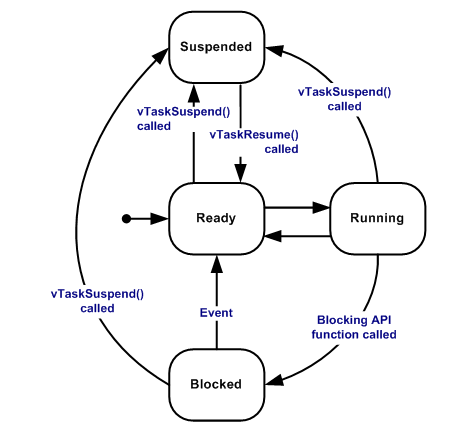
\includegraphics[width = 0.8\textwidth]{imagenes/cap1_marcoteo/TasksRTOS.png}
        \caption{Estados de las tareas en FreeRTOS \citep{rtos}.}
        \label{fig:RTOSTasks}
    \end{figure}

    \item Semáforos binarios (\textit{Binary Semaphores}): La idea general de los semáforos binarios es permitir que las tareas accedan a recursos compartidos y ejecutar tareas complejas de sincronización. Suelen usarse en conjunto con los mutex (que viene del término \textit{mutual exclusion}), los cuales evitan que se corrompan sectores de memoria cuando 2 tareas (que pueden estar ejecutándose en paralelo) quieran acceder a un espacio de memoria al mismo tiempo.
\end{itemize}

La arquitectura de un sistema basado en FreeRTOS se muestra en la figura \ref{fig:rtos}:

\begin{figure}[H]
    \centering
    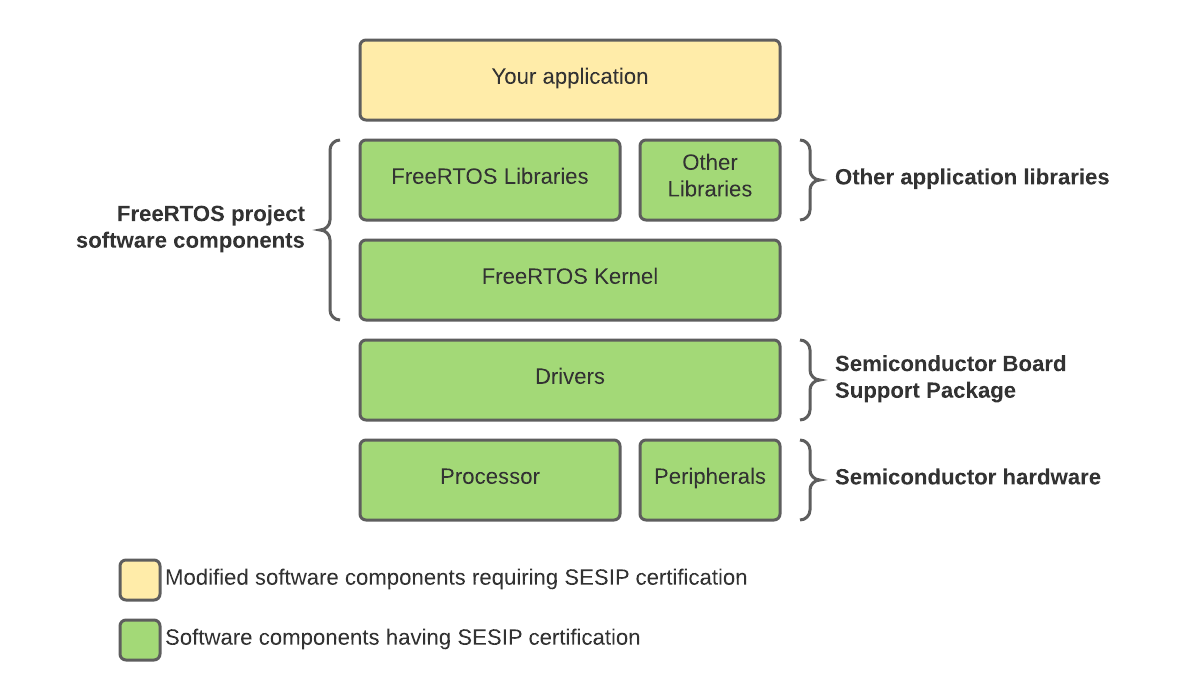
\includegraphics[width = 0.8\textwidth]{imagenes/cap1_marcoteo/FreeRTOSArch.png}
    \caption{Arquitectura de sistema embebido basado en FreeRTOS \citep{rtos}.}
    \label{fig:rtos}
\end{figure}

%SENSORES
\section{Sensores}

\subsection{Definición}

Los sensores son dispositivos capaces de detectar un parámetro físico y responder a la entrada de este fenómeno físico con una señal, usualmente eléctrica, que puede ser medida y transmitida. Usualmente se clasifican según la variable a medir, por el tipo de señal que emiten (digital o analógica, en el caso de señales eléctricas) y por su interacción con la variable a medir, siendo los activos los que generan una señal para obtener la medición y los pasivos los que responden a los cambios del medio físico. Son la base principal de todo sistema de instrumentación al representar el vínculo entre los variables físicas que se desean medir y el ser humano, cuyas capacidades sensoriales no están diseñadas para medir ciertas variables y mucho menos tomar valores y registros de las mismas.


\subsection{Características de los sensores}

\begin{itemize}
    \item Sensibilidad: Razón entre el incremento en la señal de salida del sensor y la variación en la variable medida.
    \item Resolución: Representa la variación mínima de la variable a medir que puede ser detectada por el sensor.
    \item Rango: Representa el conjunto de valores comprendidos entre el límite superior e inferior de la capacidad del instrumento de medición. Este espectro suele representarse mediante los valores extremos.
    \item Temperatura de operación: Rango de temperaturas dentro del cual el comportamiento del sensor es el esperado dentro de un límite de error.
    \item Frecuencia de respuesta o ancho de banda: Rango de valores en el espectro de frecuencia dentro de los cuales los sensores son capaces de obtener mediciones de la variable de interés. Esta característica es particularmente importante en ensayos de vibración y ensayos dinámicos.
\end{itemize}

\subsection{Sensores de interés para el Monitoreo de Salud Estructural}
\label{subsec:sensmonitoreo}

En el campo de la monitorización de salud estructural (SHM), existen varios tipos de sensores que se utilizan comúnmente. Algunos de los sensores más utilizados en SHM son los siguientes:

    \begin{itemize}
        \item Deformación: Estos sensores miden la deformación o la tensión en la estructura. Pueden incluir galgas extensiométricas, sensores de fibra óptica o sensores de cable extensométrico.
        \item Temperatura:  Estos sensores miden la temperatura ambiente o la temperatura de la estructura. Son útiles para evaluar el efecto del calor en el comportamiento estructural y detectar anomalías relacionadas con cambios térmicos. Se suelen utilizar los siguientes tipos:
        \begin{itemize}
            \item Termopares: consisten en dos cables de diferente material metálico unidos en un extremo. La diferencia de temperatura entre los extremos genera una pequeña corriente eléctrica que se puede medir y relacionar con la temperatura.
             \begin{figure}[H]
                \centering
                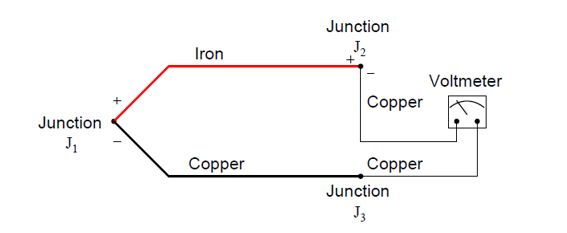
\includegraphics[width = 0.7\textwidth]{imagenes/cap1_marcoteo/termocupla-con-voltimetro.png}
                \caption{Esquema general de funcionamiento de un termopar \citep{dunn2005introduction}.}
                \label{fig:termopar}
            \end{figure}
            \item Termistores: Utilizan materiales semiconductores cuya resistencia eléctrica cambia con la temperatura. 
            \item Microelectromecánicos (MEMS): Suelen utilizar el efecto termoeléctrico o la variación de las propiedades eléctricas de los materiales con la temperatura para medir y cuantificar los cambios térmicos.
            \begin{figure}[H]
                \centering
                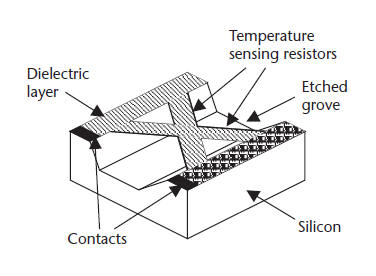
\includegraphics[width = 0.7\textwidth]{imagenes/cap1_marcoteo/TempMEMS.png}
                \caption{Esquema general de un sensor de temperatura de tecnología MEMS \citep{dunn2005introduction}.}
                \label{fig:temp-MEMS}
            \end{figure}
        \end{itemize}

        \item Humedad: Los sensores de humedad se utilizan para medir la humedad relativa o la presencia de agua en la estructura. Son particularmente útiles para evaluar el grado de corrosión en estructuras metálicas.
        \begin{itemize}
            \item Capacitivos: utilizan la capacidad dieléctrica de un material sensible a la humedad para medir el contenido de agua en el aire o en el suelo. El cambio en la capacidad dieléctrica se traduce en una señal de salida proporcional a la humedad relativa.
            \begin{figure}[H]
                \centering
                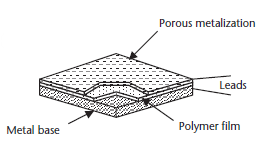
\includegraphics[width = 0.7\textwidth]{imagenes/cap1_marcoteo/HigrometroCapacitivo.png}
                \caption{Esquema general de un sensor de humedad capacitivo \citep{dunn2005introduction}.}
                \label{fig:hig-cap}
            \end{figure}
            \item Resistivos: Utilizan un material sensible a la humedad, como una película polimérica o un material cerámico, cuya resistencia eléctrica varía con la humedad.
            \begin{figure}[H]
                \centering
                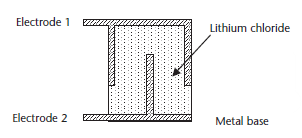
\includegraphics[width = 0.7\textwidth]{imagenes/cap1_marcoteo/HigrometroResistivo.png}
                \caption{Esquema general de un sensor de humedad resistivo \citep{dunn2005introduction}.}
                \label{fig:hig-res}
            \end{figure}
            \item Microelectromecánicos (MEMS): suelen utilizar una capa de material sensible a la humedad, como un polímero higroscópico, que experimenta cambios en sus propiedades físicas, eléctricas o capacitivas en respuesta a la humedad del ambiente. 
            \begin{figure}[H]
                \centering
                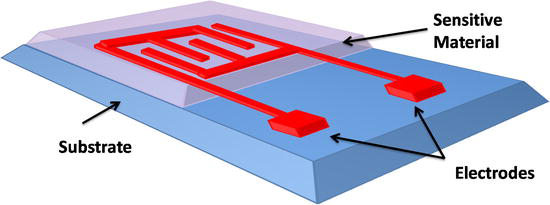
\includegraphics[width = 0.7\textwidth]{imagenes/cap1_marcoteo/HigrometroMEMS.png}
                \caption{Esquema general de un sensor de humedad de tecnología MEMS \citep{alfaifi2021mems}.}
                \label{fig:hig-mems}
            \end{figure}
        \end{itemize}

        \item Acelerómetros: Estos sensores se encargan de medir la aceleración de la estructura en una o varias direcciones. Son útiles para evaluar la respuesta dinámica de la estructura ante cargas externas, vibraciones o sismos. Existen varios tipos de acelerómetros, entre los que se encuentran:
        
        \begin{itemize}
            \item Piezoeléctrico: Se basan en el principio piezoeléctrico, donde un cristal piezoeléctrico genera una carga eléctrica proporcional a la aceleración aplicada. Son sensibles, ofrecen una amplia respuesta en frecuencia y son adecuados para medir tanto bajas como altas frecuencias de vibración. 
            \begin{figure}[H]
                \centering
                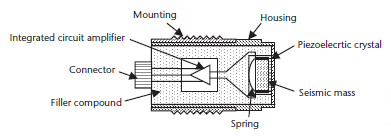
\includegraphics[width = 0.7\textwidth]{imagenes/cap1_marcoteo/AccelerometerPiezo.png}
                \caption{Esquema general de un acelerómetro piezoeléctrico \citep{dunn2005introduction}.}
                \label{fig:acc-pie}
            \end{figure}
            \item Capacitancia Diferencial: utilizan un conjunto de placas móviles y fijas separadas por una pequeña distancia. La aceleración causa un cambio en la distancia entre las placas, lo que a su vez modifica la capacitancia del dispositivo. Este cambio en la capacitancia es proporcional a la aceleración.
            \item Microelectromecánicos (MEMS): Se basan en el desplazamiento de una masa suspendida mediante resortes micromecánicos. Son pequeños, económicos y se utilizan ampliamente en aplicaciones de monitoreo estructural debido a su tamaño compacto y bajo consumo de energía.
            \begin{figure}[H]
                \centering
                \begin{minipage}{0.45\textwidth}
                    \centering
                    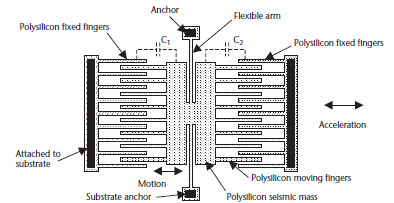
\includegraphics[width=1\textwidth]{imagenes/cap1_marcoteo/AccelerometerMEMS.png}
                    \caption{Esquema general de un acelerómetro de tecnología MEMS \citep{dunn2005introduction}.}
                    \label{fig:acc-mems1}
                \end{minipage}
                \hfill
                \begin{minipage}{0.45\textwidth}
                    \centering
                    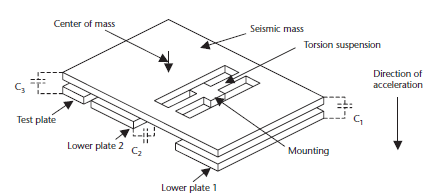
\includegraphics[width=1\textwidth]{imagenes/cap1_marcoteo/AccelerometerMEMS2.png}
                    \caption{Acelerómetro microelectromecánico \citep{dunn2005introduction}.}
                    \label{fig:acc-mems2}
                \end{minipage}
            \end{figure}


            \item Balance de fuerzas: Este tipo de acelerómetro consiste en un detector de posición, un amplificador y un sistema electromecánico de posicionamiento. El sistema convierte una fuerza mecánica en una corriente proporcional que se convierte en una fuerza en dirección contraria para contrarestar el movimiento de la masa suspendida. 
            
            El detector de posición registra la posición de una masa acoplada al generador de fuerza. Un cambio inducido externamente en la posición de la masa resulta en una combinación de la salida del detector de posición y del amplificador de tal forma que el generador de fuerza o motor de torque lleve la masa de vuelta a su posición original. La salida del sensor es una medida de la corriente a través del generador de fuerza o motor, siendo esta corriente proporcional a la fuerza de restauración que es igual a la fuerza de entrada a través de la masa calibrada.

            \begin{figure}[H]
                \centering
                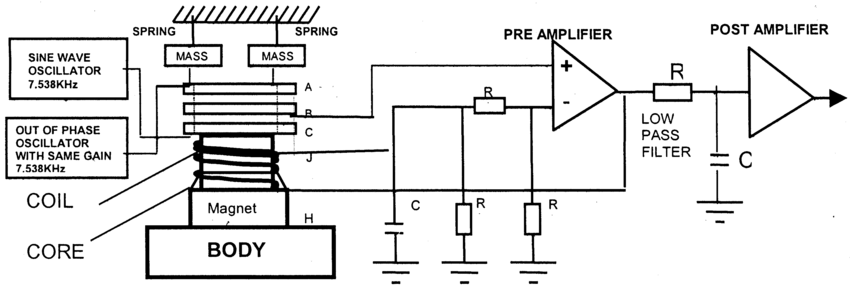
\includegraphics[width = 0.7\textwidth]{imagenes/cap1_marcoteo/Block-diagram-of-force-balance-accelerometer.png}
                \caption{Esquema general de un acelerómetro por balance de fuerza \citep{balanceforce}.}
                \label{fig:acc-fba}
            \end{figure}

            Si no hay aceleración en la masa, la corriente a través del motor de torque es nula. El amortiguamiento es controlado por un condensador y se coloca en paralelo con la resistencia de muestreo.
        \end{itemize}

    \end{itemize}

\subsection{Fusión de sensores}
\label{subsec:sensorfusion}

La fusión de sensores consiste en combinar la información de múltiples sensores para obtener una medida más precisa y confiable de la variable de interés \citep{lamkin2019sensors}. La fusión de sensores puede mejorar la precisión, la confiabilidad y la robustez de las mediciones, ayudando también a reducir la incertidumbre y el ruido presente en los datos. La combinación de estas mediciones se puede hacer de distintas formas, las cuales se mencionan a continuación:

\begin{itemize}
    \item Sensores redundantes: Todos los sensores proporcionan la misma información sobre la variable de interés. La redundancia de sensores puede mejorar la confiabilidad y la precisión de las mediciones, ya que si un sensor falla, los otros sensores pueden seguir proporcionando datos.
    
    \item Sensores complementarios: Los sensores proporcionan información independiente o complementaria sobre la variable de interés. Al combinar la información de sensores complementarios, se puede obtener una medida más precisa y completa de la variable de interés.
    \item Sensores coordinados: Los sensores recopilan información sobre la variable de interés de forma secuencial. 
\end{itemize}

La fusión de sensores permite obtener información a partir de varios sensores que no está disponible a través de un sensor en específico, siendo necesario recopilar distintas variables físicas para reconstruir la variable de interés. La fusión de sensores es una técnica comúnmente utilizada en aplicaciones de monitoreo estructural, robótica, navegación y sistemas de control, entre otros.

\subsubsection{Estimación de ángulos}

Una de las variables físicas que suele obtenerse a partir de la fusión de información de varios sensores es la inclinación. Existen distintos métodos, cada uno con sus ventajas y deficiencias, para obtener una estimación de la inclinación de un sistema a partir de mediciones de acelerómetros, giróscopos y magnetómetros. Algunos de los métodos más comunes son:

\begin{itemize}
    \item Integración de la medición del giróscopo: Se utiliza la medición de la velocidad angular del giróscopo para estimar la orientación del sistema. Sin embargo, la integración de la velocidad angular puede acumular errores y derivar en una estimación incorrecta de la orientación.
    \item Estimación por trigonometría: Se utilizan las mediciones de los acelerómetros y magnetómetros para estimar la orientación del sistema a partir de cálculos trigonométricos. Este método puede ser sensible a errores en las mediciones y a la presencia de campos magnéticos externos.
	\item Filtro de Kalman: El Filtro de Kalman es uno de los algoritmos de estimación más utilizados en la industria. En el caso de la estimación de inclinación, combina mediciones de sensores con un modelo dinámico del sistema para obtener una estimación precisa de la orientación. El filtro de Kalman es particularmente útil para fusionar mediciones de acelerómetros, giróscopos y magnetómetros y estimar la orientación en tiempo real.
	
	\item Filtro de Madgwick: El filtro de Madgwick es un algoritmo de fusión de sensores que utiliza mediciones de giroscopios, acelerómetros y magnetómetros para estimar la orientación del sistema. El filtro de Madgwick es una versión simplificada del filtro de Kalman y es ampliamente utilizado en aplicaciones de realidad virtual, aumentada y sistemas de navegación inercial.
	
    Este método, desarrollado por \cite{madgwick2010efficient}, hace uso de cuaterniones para la representación espacial. Estos son una extensión de los números complejos y se utilizan para representar rotaciones en el espacio tridimensional.

    Las representaciones tridimensionales traen problemas como el bloqueo de cardán, que consiste en la pérdida de un grado de libertad en la representación de los ángulos de Euler.

    Un cuaternión consta de cuatro componentes:

    \begin{enumerate}
        \item Parte escalar (w).
        \item Tres partes vectoriales (x, y, z).
    \end{enumerate}

    Se representan de la siguiente forma:

    \begin{equation}
        q = w + xi + yj + zk
    \end{equation}

    El filtro emplea esta representación para evitar los problemas asociados con la representación tridimensional de los ángulos de Euler, permitiendo que los datos de aceleración y magnetómetro se utilicen en un algoritmo de descenso de gradiente derivado de forma analítica y optimizado para calcular la dirección del error de medición del giroscopio como una derivada de cuaternión.

    El algoritmo utiliza una combinación de la información proporcionada por los giroscopios (para estimar la velocidad angular) y los acelerómetros y magnetómetros (para estimar la gravedad y el vector magnético terrestre) para calcular la orientación.
\end{itemize}

\section{Sensores inteligentes}

\subsection{Definición:}

Si bien los sensores por sí mismos han permitido un rápido y sostenido desarrollo en todos los ámbitos de la instrumentación en distintas áreas de la industria, el advenimiento de la era digital y la miniaturización de los componentes ha impulsado cambios en la manera en la que se mide hoy en día. Con el poder de cómputo actual, los sensores aumentan sus capacidades cuando son parte de un sistema más grande capaz de procesar la información que estos proveen.

Un sensor inteligente es un sistema en donde uno o varios sensores y una interfaz electrónica dedicada trabajan en conjunto. La tecnología empleada para llevar a cabo estos sistemas ha avanzado rápidamente en años recientes, lográndose obtener sistemas de un solo chip para medir temperatura o campo magnético \citep{nagayama2007structural}.


El término sensor inteligente o \textit{``smart sensor''} surgió a mediados de los años 80. La ``inteligencia'' de estos dispositivos viene dada por un microcontrolador (MCU), un procesador de señales digitales (DSP) y circuitos de aplicación específica \citep{frank2002understanding}. Posteriormente, en el año 1998, el \textit{IEEE} en su estándar \textit{Networked smart transducer interface standard 1451} definió un \textit{``smart sensor''} como un transductor que provee funciones más allá de las necesarias para generar y representar una cantidad medida \citep{song2008understanding}.

\subsection{Características:}

Un sensor inteligente suele tener 5 características esenciales, las cuales se resumen a continuación:

\begin{itemize}
    \item Microprocesador integrado: Es lo que diferencia un sensor común de un sensor inteligente, siendo este el encargado de hacer los cálculos necesarios, guardar los datos de forma local, enviar resultados y coordinar las tareas a ejecutarse. 
    
    \item Capacidades de medición: La principal característica de un sensor es su capacidad de convertir una variable física en algún tipo de señal que pueda ser posteriormente procesada, en este caso por el microprocesador integrado, siendo el sensor el vínculo entre el procesador y los fenómenos físicos de interés. Un sensor inteligente, también llamado nodo, puede constar de varios sensores que miden distintas variables.
    
    \item Comunicación inalámbrica: En gran medida, se busca que los sensores inteligentes sean capaces de reemplazar los actuales sistemas de medición cableados, permitiendo esto la expansión del sistema de medición a un bajo costo, además de las capacidades de transmisión que ofrecen alternativas como láser, infrarrojo, o incluso ondas de radio y telefonía.
    
    \item Alimentación autónoma: Con frecuencia los sensores inteligentes son alimentados de forma autónoma con baterías, en particular en aplicaciones de difícil acceso, como es el caso de algunas estructuras civiles. Si bien esto representa un desafío, la logística y los requerimientos asociados a conectar todo un sistema mallado de sensores a la red eléctrica atenta en contra de la facilidad de instalación y mantenimiento de un sistema inteligente.
    
    \item Bajo costo: Una de las características más importantes que se busca obtener al hacer uso de sistemas basados en sensores inteligentes es reducir los costos generados por un sistema basado en sensores comunes. Tecnologías como MEMS (\textit{Micro electro-mechanical systems}) han logrado reducir de forma considerable el tamaño y el costo por su producción en masa basada en semiconductores. Esta característica permite que redes densas de sensores sean implementadas en estructuras civiles.
\end{itemize}


\section{Monitoreo}

El monitoreo se refiere a la observación continua de un proceso, medición o medición para obtener información sobre su estatus y comportamiento. Estos datos pueden ser procesados y analizados posteriormente para detectar cambios, anomalías, fallas y tomar decisiones de control. Se puede subdividir en dos enfoques:

\subsection{Monitoreo cableado} Involucra el uso de cables que comunican los dispositivos de adquisición o medición y el sistema central de procesamiento o almacenamiento. La información viaja a través de estos cables que pueden ser coaxiales, fibra óptica, de par trenzado, entre otros. 

\subsection{Monitoreo inalámbrico} Involucra el uso de redes de comunicaciones inalámbricas para el envío de los datos adquiridos por los dispositivos de medición. Los sensores deben contar con un transmisor de datos, enviando los datos en forma de ondas electromagnéticas hasta el receptor, el cual debe encargarse de recibir y decodificar estas señales en la estación central. Algunas de las tecnologías más utilizadas para el monitoreo inalámbrico son WiFi, Bluetooth, Zigbee, LoRa y la red celular. 

\begin{table}[H]
    \centering
    \caption{Ventajas y desventajas de los enfoques de monitoreo.}
    \label{tab:monitoreo}
    \resizebox{0.9\textwidth}{!}{%
    \begin{tabular}{|P{0.3\textwidth}|P{0.3\textwidth}|P{0.3\textwidth}|}
    \hline
    \textbf{Monitoreo} & \textbf{Ventajas} & \textbf{Desventajas} \\ \hline
    \textbf{Cableado} & \begin{itemize}
        \item Confiabilidad.
        \item Seguridad.
        \item Gran ancho de banda.
    \end{itemize}  & \begin{itemize}
        \item Movilidad limitada
        \item Instalación compleja
        \item Costo elevado.
    \end{itemize} \\ \hline
    \textbf{Inalámbrico} & \begin{itemize}
        \item Flexibilidad y movilidad.
        \item Fácil instalación
        \item Escalabilidad y bajo costo.
    \end{itemize} & \begin{itemize}
        \item Complejidad elevada.
        \item Posibilidad de interferencia.
        \item Ancho de banda limitado.
    \end{itemize} \\ \hline
    \end{tabular}%
    }
\end{table}


\section{Sistemas de adquisición de datos}

\subsection{Definición y esquema general} Un sistema de adquisición de datos o DAQ (\textit{Data acquisition systems})  consiste en un sistema que incluye sensores, un computador o procesador y software de adquisición de datos integrado. Es capaz de obtener, almacenar, visualizar y procesar los datos de interés. Fueron diseñados con el fin de obtener información sobre algún fenómeno físico aislado o parte de un proceso o sistema más grande, siendo la interfaz entre las variables físicas y el monitoreo del sistema en cuestión.

\subsection{Acondicionamiento de señales} Las señales obtenidas por el DAQ presentan ruido y pueden verse atenuadas por el canal de comunicación que comunica los sensores con el dispositivo de almacenamiento y procesamiento, es por esto que es preciso filtrar y amplificar la señal previo a su entrada al sistema de adquisición, o en su defecto, previo a su almacenamiento y procesamiento.

\subsection{DAQ basados en MCU} Dadas las capacidades de procesamiento y comunicación de los microcontroladores en la actualidad, es común ver sistemas de adquisición de datos basados en microcontroladores, haciendo uso de sus periféricos para leer el voltaje de los sensores usando el ADC integrado en los mismos, o a su vez, interpretando las señales digitales provenientes de sensores que utilizan protocolos de comunicación serial.


\section{Sistemas de comunicaciones inalámbricos}

\subsection{Características y conceptos básicos}

Un sistema de comunicaciones inalámbrico es un sistema de transmisión de información que utiliza ondas electromagnéticas para transmitir datos sin la necesidad de cables físicos. En lugar de utilizar conexiones alámbricas, se emplean tecnologías de radio, microondas, infrarrojos u otras frecuencias electromagnéticas para la transmisión de datos de manera inalámbrica. Los elementos principales de un sistema de comunicaciones se describen a continuación:

\begin{itemize}
    \item Transmisor: Se refiere al dispositivo o sistema que se encarga de convertir una señal o información en una forma adecuada para su transmisión a través de un medio de comunicación. El transmisor realiza procesos de modulación y amplificación de la señal para adaptarla a las características del canal de transmisión del sistema.

    \item Canal de transmisión: Es el medio físico o inalámbrico a través del cual se envía la señal o información desde el transmisor al receptor. En el caso inalámbrico, este canal es el aire. Puede introducir distorsiones, atenuación, retardos o interferencias en la señal transmitida.

    \item Receptor: Dentro de un canal de comunicaciones, es el dispositivo o sistema que recibe la señal transmitida a través del canal de transmisión y la convierte nuevamente en una forma adecuada para su interpretación o uso. El receptor realiza procesos de demodulación, filtrado y amplificación de la señal recibida para recuperar la información original.

    \item Interferencias: Las interferencias se refieren a señales o perturbaciones no deseadas que afectan la señal transmitida en el canal de comunicación. Estas interferencias pueden ser causadas por fuentes externas, como señales electromagnéticas de otros dispositivos o fenómenos naturales, o por interferencias internas generadas por componentes electrónicos o ruido en el propio sistema de comunicación. Las interferencias pueden degradar la calidad de la señal, causar errores en la transmisión o incluso impedir la correcta recepción de la información.

    \item Ruido: Puede definirse como una señal o perturbación no deseada que se superpone a la señal útil durante la transmisión o recepción de datos. El ruido puede ser generado internamente en los componentes electrónicos, introducido por fuentes externas o ser el resultado de las características inherentes del canal de transmisión. 

\end{itemize}

\subsection{Protocolos de comunicación para distancias cortas}

\begin{itemize}
    \item WiFi (\textit{Wireless Fidelity}): Es el protocolo de comunicación inalámbrica más popular. Consiste en una tecnología inalámbrica que hace uso del estandar 802.11 del IEEE a través de frecuencias como 2.4 GHz y 5 GHz. Suele tener un rango entre 20 y 40 metros y se caracteriza por velocidades de transmisión muy altas, de hasta 600 Mbps.
    
    \item Bluetooth: Uno de los medios de comunicación más utilizados en la actualidad. Bluetooth es una tecnología utilizada para el intercambio de datos a distancias cortas (con un rango entre 50 y 100 metros) que hace uso de frecuencias entre 2.4 a 2.485 GHz. Tiene una velocidad máxima de 1 Mbps y es ampliamente utilizado para transferencia de datos entre dispositivos móviles.
    
    \item Zigbee: Es un estándar de comunicación inalámbrica de corto alcance y bajo consumo de energía diseñado para aplicaciones de Internet de las cosas (IoT). Utiliza la tecnología de radio de baja potencia y bajo consumo para permitir la comunicación inalámbrica entre dispositivos Zigbee, como sensores, actuadores y controladores. Zigbee opera en las bandas de frecuencia de 2.4 GHz, 900 MHz u 868 MHz y se basa en una topología de malla, lo que significa que los dispositivos pueden comunicarse directamente entre sí o a través de otros dispositivos Zigbee cercanos. 
    
    \item MQTT (Message Queuing Telemetry Transport): MQTT es un protocolo ligero basado en el modelo ``publish/subscribe'', diseñado por ingenieros de la IBM y Arcom Systems específicamente para aplicaciones del internet de las cosas (\textit{Internet of Things}), requiriendo poco ancho de banda y siendo fiable en redes inestables. Consiste en un broker, encargado de gestionar los datos, al cual se conectan los clientes, los cuales pueden publicar (enviar datos), o suscribirse a un tópico del broker (acceder a los datos que se publicaron a ese tópico desde algún cliente).
    
    \begin{figure}[H]
        \centering
        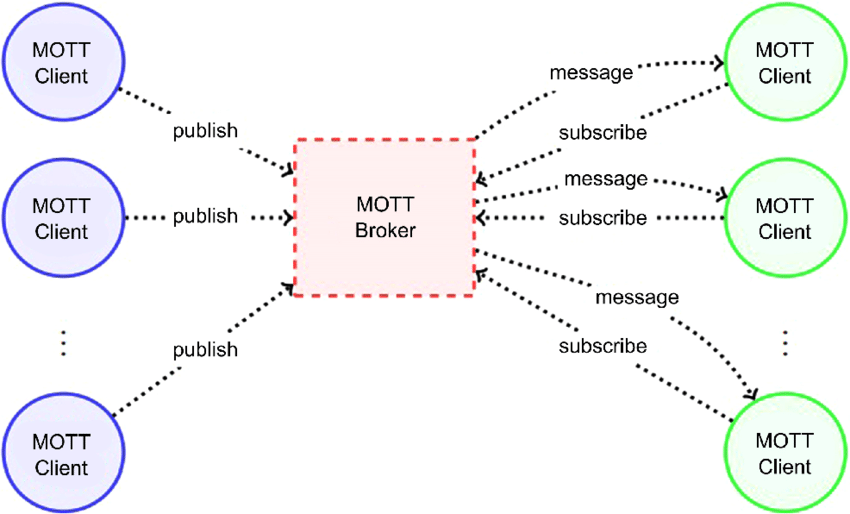
\includegraphics[width = 0.7\textwidth]{imagenes/cap1_marcoteo/MQTT-protocol-model.png}
        \caption{Esquema general del protocolo MQTT \citep{aloufi2020hybrid}.}
        \label{fig:mqtt}
    \end{figure}
    
\end{itemize}

\subsection{Protocolos de comunicación de larga distancia}

\begin{itemize}

    \item NB-IoT: NB-IoT (\textit{Narrowband Internet of Things}) es un estándar de comunicación de larga distancia y bajo consumo de energía para dispositivos IoT. Utiliza la infraestructura de redes celulares existentes y opera en bandas de frecuencia estrechas para proporcionar conectividad de bajo ancho de banda y larga duración de la batería.
    \item Sigfox: Es una tecnología de comunicación de larga distancia y bajo consumo de energía diseñada para el IoT (\textit{Internet of Things}). Utiliza una red de bajo consumo de energía y bajo costo para transmitir pequeñas cantidades de datos de forma eficiente. Sigfox es utilizado en aplicaciones de seguimiento de activos, monitoreo ambiental y aplicaciones industriales. 
    \item LoRa: LoRa (cuyas siglas provienen de \textit{Long Range}) es una tecnología de comunicación inalámbrica de largo alcance y baja potencia diseñada para aplicaciones de IoT y M2M (\textit{machine-to-machine}). Se basa en el estándar LoRaWAN (\textit{LoRa Wide Area Network}) y utiliza una modulación de espectro ensanchado para lograr una mayor cobertura y capacidad de penetración en comparación con otras tecnologías inalámbricas. LoRa opera en las bandas de frecuencia libre de licencia y puede proporcionar alcances de varios kilómetros en áreas urbanas y aún mayores en áreas rurales. Debido a su bajo consumo de energía, es adecuado para dispositivos de batería de larga duración y aplicaciones de bajo ancho de banda.
\end{itemize}

Dependiendo de la aplicación se debe escoger la tecnología más conveniente. Esto dependerá de la distancia entre los dispositivos que recolectan datos y la estación base, la naturaleza de los datos a enviar y las restricciones de tiempo impuestas por el sistema en estudio. A continuación se presenta un gráfico comparativo entre las distintas tecnologías:

\begin{figure}[H]
    \centering
    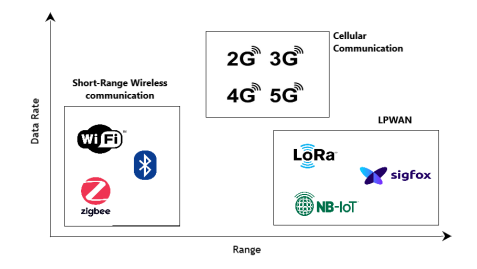
\includegraphics[width = 0.8\textwidth]{imagenes/cap1_marcoteo/CommPrtocolsComparison.png}
    \caption{Esquema comparativo entre distintas tecnologías tomando en cuenta el rango de alcance y el ancho de banda \citep{khorsandi2023performance}.}
    \label{fig:commcomparison}
\end{figure}

\subsection{Protocolo LoRa}
\label{sec:protocololora}

Esta tecnología fue desarrollada en Francia en el año 2012 por la empresa francesa Semtech. Es el tipo de modulación utilizado entre dos dispositivos LoRa o entre un \textit{end-device} y un \textit{gateway}. 

El récord mundial para una transmisión LoRa es de 832 km, logrado por Thomas Telkamp en la banda EU868 utilizando 25 mW / 14 dBm \citep{montagny2021lora}.

Suelen confundirse los términos LoRa y LoRaWAN (Long Range Wide Area Network). LoRa se refiere al tipo de modulación mientras que LoraWAN es una extensión del protocolo LoRa que da la capacidad de conectar los dispositivos a un servidor para servir de interfaz con el usuario final. Puede definirse LoRaWAN como una arquitecturade red que consta de dispositivos finales, gateways y servidores.

\begin{itemize}
    \item Funcionamiento: LoRa utiliza una técnica de modulación de espectro ensanchado llamada modulación de espectro ensanchado de baja potencia (CSS, por sus siglas en inglés). Esta técnica permite que las señales de radio se propaguen a distancias más largas y atraviesen obstáculos, lo que proporciona una mayor cobertura en comparación con otras tecnologías inalámbricas.
    
    Para transmitir los datos hace uso de ``Chirps'' (Compressed High Intensity Radar Pulse por sus siglas en inglés), de donde viene su nombre CSS. Esta señal, que puede observarse en la figura \ref{fig:chirp}. Un chirp es una señal que varía en frecuencia linealmente con el tiempo.

    \begin{figure}[H]
        \centering
        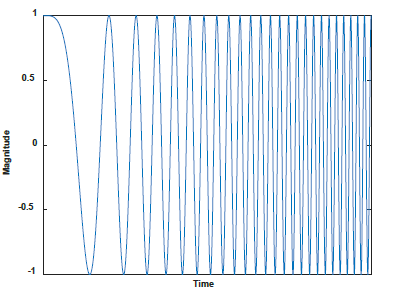
\includegraphics[width = 0.7\textwidth]{imagenes/cap1_marcoteo/ChripSignal.png}
        \caption{Señal chirp utilizada para la tranmisión CSS \citep{aloufi2020hybrid}.}
        \label{fig:chirp}
    \end{figure}

    \item Ancho de banda: Uno de los parámetros más importantes dentro de un canal de comunicaciones. Puede definirse como la cantidad de espectro de frecuencia ocupado por una señal de transmisión. Es un parámetro importante que determina la capacidad de transmisión de datos y la eficiencia espectral de la comunicación. En LoRa, el ancho de banda se puede configurar en diferentes opciones, como 125 kHz, 250 kHz y 500 kHz. La elección del ancho de banda afecta directamente la velocidad de transmisión de datos y el alcance de la comunicación.
    
    \begin{figure}[H]
        \centering
        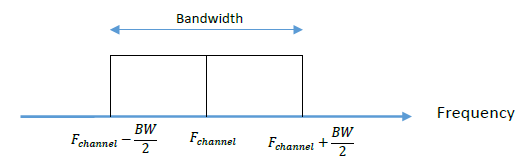
\includegraphics[width = 0.8\textwidth]{imagenes/cap1_marcoteo/AnchodeBandaLoRa.png}
        \caption{Ancho de banda representado en el espectro \citep{aloufi2020hybrid}.}
        \label{fig:anchobanda}
    \end{figure}

    \item Factor de propagación: El factor de propagación (Spreading Factor) se refiere a un parámetro que determina la velocidad de transmisión de datos y la robustez de la comunicación.

    El spreading factor se representa como un número entero que varía típicamente de 7 a 12 en la tecnología LoRa. Un spreading factor más bajo indica una velocidad de transmisión de datos más alta, pero con menor alcance y capacidad de penetración de la señal. Por otro lado, un factor de propagación más alto proporciona un mayor alcance de comunicación, pero con una velocidad de transmisión de datos más baja.
    
    En LoRa cada símbolo representa un número de bits transmitidos. Por tanto, se define la siguiente regla:

    \begin{equation}
        \text{Número de bits transmitidos en un símbolo} = \text{Factor de propagación}
    \end{equation}

     Para un SF10, un símbolo o \textit{Chirp} representará 10 bits. Esto se observa claramente en la figura \ref{fig:spreadingfactor}:

     \begin{figure}[H]
        \centering
        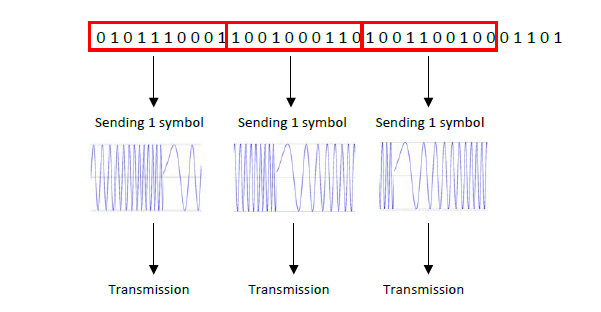
\includegraphics[width = 0.8\textwidth]{imagenes/cap1_marcoteo/SpreadingFactor.png}
        \caption{Representación de símbolos en una transmisión LoRa \citep{aloufi2020hybrid}.}
        \label{fig:spreadingfactor}
    \end{figure}
    
    \item Potencia: Los dispositivos LoRa generalmente permiten ajustar la potencia de transmisión de la señal. Esto proporciona flexibilidad para adaptarse a diferentes escenarios y requisitos de alcance. Por ejemplo, en áreas densamente pobladas o con obstáculos, se puede aumentar la potencia de transmisión para superar la atenuación de la señal y mejorar la cobertura. En Venezuela la potencia máxima de transmisión está regulada por CONATEL, siendo en la banda libre de telemetría alrededor de los 470 MHz de 250 mW (24 dBm) \citep{conatel}.
    
    \item Rango: El rango de transmisión en LoRa puede variar desde unos pocos cientos de metros hasta varios kilómetros, dependiendo de los factores mencionados anteriormente. Utilizando técnicas como factor de propagación alto, potencia de transmisión adecuada y condiciones de propagación favorables, es posible lograr comunicaciones en rangos de varios kilómetros en entornos abiertos y sin obstrucciones.
    
    \item Tiempo de transmisión: El tiempo de transmisión de cada símbolo depende del factor de propagación. Es decir, a mayor SF, el tiempo de transmisión será mayor manteniendo el ancho de banda igual. Tomando esto en cuenta se tiene la siguiente ecuación:
    
    \begin{equation}
        T_{symbol} = \frac{2^{SF}}{\text{Ancho de banda}}
    \end{equation}

    \item Forma de la trama: Las tramas de LoRa, como la que se muestra en la figura \ref{fig:trama},siguen una estructura predefinida que consta de 4 partes:
    
    \begin{figure}[H]
        \centering
        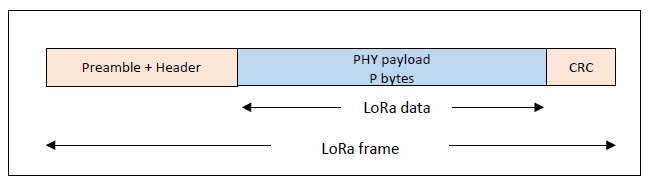
\includegraphics[width = 0.7\textwidth]{imagenes/cap1_marcoteo/FormatramaLora.png}
        \caption{Forma de la trama LoRa \citep{aloufi2020hybrid}.}
        \label{fig:trama}
    \end{figure}

    \begin{enumerate}
        \item Preámbulo (\textit{Preamble}): Secuencia de bits que se utiliza para sincronizar el receptor con la transmisión y permitir la detección y sincronización de la trama.
        \item Encabezado (\textit{Header}): Se puede utilizar un encabezado adicional para incluir información adicional sobre la trama, como la dirección de origen o destino, los identificadores de servicio, etc. Puede ser generada de forma automática o programada.
        \item Carga útil (\textit{Payload}): Campo principal de la trama que contiene los datos que se van a transmitir. 
        \item CRC (\textit{Cyclic Redundancy Checking}): Campo que contiene un código de detección de errores para verificar la integridad de la trama recibida. El receptor realiza un cálculo CRC sobre los datos recibidos y compara el resultado con el valor de CRC incluido en la trama. Si el valor calculado y el valor de CRC coinciden, se asume que la trama se recibió sin errores
    \end{enumerate}



    \item Tasa de codificación (CR): En LoRa, se utiliza la codificación de corrección de errores de tipo ``\textit{forward error correction}'' (FEC), que permite detectar y corregir errores en la recepción de los datos. El coding rate especifica la cantidad de bits redundantes que se agregan a los datos para mejorar la confiabilidad de la comunicación. En el caso de un $CR = 4 / 8$, 8 bits son transmitidos mientras que solo 4 bits contienen información útil.
    
    
    \item Consumo de energía: El protocolo se caracteriza por tener un bajo consumo de energía, permitiendo ser empleado en dispositivos a baterías para envío de datos periódicos. Esto se traduce en velocidades bajas de tranmisión y cargas útiles (\textit{payloads}) menores a los encontrados en otras tecnologías, sin embargo, la relación entre las distancias largas a cubrir y los algoritmos de detección permiten que para ciertas aplicaciones este protocolo sea el ideal, razón por la cual se ha convertido en uno de los más utilizados en años recientes.
\end{itemize}

\section{Procesamiento digital de señales:}

El procesamiento digital de señales (DSP por sus siglas en inglés) es un proceso que involucra la manipulación de señales de distinta naturaleza en un procesador o computador. La necesidad de este procesamiento surge por la necesidad de mejorar, cambiar o mostrar los datos obtenidos de señales reales en distintas formas mediante métodos matemáticos \citep{proakisDSP}.

En gran cantidad de aplicaciones, los procesadores analógicos están siendo reemplazados por chips de DSP, esto debido a la disminución en el costo además de la capacidad de procesamiento que sigue en aumento. Si bien se puede hacer procesamiento digital con cualquier procesador o microcontrolador, estos chips están diseñados para realizar cálculos matemáticos y llevar a cabo algoritmos de procesamiento de forma eficiente. 

En el contexto de SHM, el DSP es necesario una vez los datos fueron adquiridos en campo, siendo esta herramienta la que permite realizar un estudio exhaustivo de las señales adquiridas por los sensores en el dominio de la frecuencia, siendo este estudio uno de los más importantes y utilizados en esta área.

\subsection{Estudio en el dominio de la frecuencia} El estudio de señales en el dominio de la frecuencia se remonta al siglo XIX y está estrechamente relacionado con los trabajos del matemático francés Jean-Baptiste Joseph Fourier. Desde entonces, el impacto que ha tenido en la ingeniería y las ciencias es notable. En nuestro día a día, muchos de los sistemas de uso diaro hacen uso, de alguna forma u otra, del concepto inicial planteado por Fourier. 

En el SHM, el análisis de frecuencia también desempeña un papel importante. En el monitoreo de salud estructural se utilizan técnicas de análisis de frecuencia, como la transformada de Fourier, para identificar patrones y características de frecuencia en las señales registradas por los sensores. Esto permite detectar cambios en las propiedades dinámicas de la estructura, como frecuencias naturales, modos de vibración, y cambios en la rigidez o la masa.

Como se planteó anteriormente, al estudiar el dominio de la frecuencia en el SHM, se pueden identificar patrones anómalos, compararlos con datos de referencia y tomar medidas preventivas o correctivas para garantizar la integridad y la seguridad de la estructura.

Los análisis de vibración suelen analizarse utilizando la Transformada Rápida de Fourier (FFT por sus siglas en inglés), un algoritmo computacional que ha permitido hacer uso de la Transformada de Fourier en todo tipo de aplicaciones. Para entender la FFT, es necesario definir el desarrollo matemático de la Transformada de Fourier:

% When we are dealing with random signal, normally we will use Power Spectrum Density (PSD). For these types of post processing, we may want to properly set frequency resolution, windowing type, averaging, etc to be able to obtain meaningful result. For even deeper analysis, we can go for Frequency Response Function (FRF/Transmissibility) or even Waterfall (Order Tracking) analysis. By doing this, we may be able to see the dynamic characteristic of our structure (resonance, damping, Q factor, etc). For short duration transient shock pulse, sometimes we want to use Shock Response Spectrum (SRS) to check the frequency content. For fatigue analysis, especially for random signal, we can perform rainflow counting analysis. Combining this with S-N fatigue curve, we may be able to calculate the fatigue damage.

\subsection{Transformada de Fourier}
Es una herramienta matemática utilizada para descomponer una función en sus componentes de frecuencia. Permite analizar una señal en el dominio de la frecuencia y determinar las diferentes frecuencias que la componen. Se ha convertido en una de las principales herramientas para resolver muchos desfíos de la comunidad científica, siendo su aplicación más conocida en el análisis de sistemas lineales invariantes en el tiempo. Se define matemáticamente como sigue:

\begin{equation}
    F(k) = \int_{-\infty}^{\infty} f(x) e^{-2\pi i k x} dx
\end{equation}

En la figura \ref{fig:fourier} se observa como una señal compuesta por distintas sinusoidales que varían en amplitud y frecuencia, son representadas en el dominio de la frecuencia como componentes aislados. 

\begin{figure}[H]
    \centering
    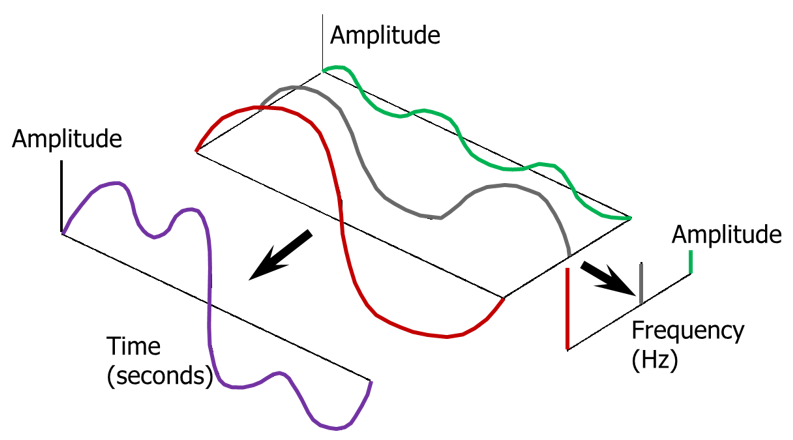
\includegraphics[width = 0.7\textwidth]{imagenes/cap1_marcoteo/FourierTRansform.png}
    \caption{Descomposición de señal temporal en el espectro de frecuencia \citep{siemens2019}.}
    \label{fig:fourier}
\end{figure}

% \subsection{Transformada de ondículas (Wavelets)} La teoría de la transformada ondícula fue desarrollada por los investigadores franceses J. Morlet y A. Grossmann en los años setenta con el fin de dar solución a problemas abstractos relacionados con geofísica. Nadie anticipó las importantes aplicaciones que luego tendría en el análisis y procesamiento de señales.

% En los últimos años ha levantado interés entre distintas áreas de investigación, siendo el SHM una de ellas. Numerosos artículos, recopilados en trabajos de autores como \cite{taha2006wavelet} y \cite{kankanamge2020application}, estudian el uso de la transformada de ondícula en aplicaciones de monitoreo de salud estructural como una alternativa a la comúnmente utilizada FFT. Si bien la transformada ofrece ventajas a la hora de obtener información relevante, no ha sido adoptada en su mayoría por la complejidad del desarrollo matemático que requiere.



\subsection{Transformada Rápida de Fourier} Tal vez uno de los algoritmos más importantes de todos los tiempos. Descrita por algunos de sus autores principales, la transformada rápida de Fourier  (FFT) es una herramienta computacional que facilita el análisis de señales en el espectro de la frecuencia mediante el uso de computadores digitales. Ejecuta la transformada discreta de fourier de una forma más eficiente 

La transformada de Fourier exige un cálculo que puede ser computacionalmente costoso, especialmente cuando se trata de muchos puntos. Es ahí donde la FFT explota las simetrías matemáticas para lograr disminuir el cálculo de una complejidad $O(N^2)$, una función prácticamente lineal en ``n'', a mayor ``n'' el valor no crece tan rápidamente que la expresión cuadrática origianl. Siendo N es el número de datos, a una complejidad de $O(N\log_{N})$. Se describe matemáticamente utilizando la siguiente expresión:

\begin{equation}
    X[k] = \sum_{n=0}^{N-1} x[n] \cdot e^{-j 2 \pi k n / N}
\end{equation}

Donde:

\begin{itemize}
    \item X[k] = Muestra ``k'' de la transformada discreta de Fourier (DFT).
    \item x[n] = Muestra ``n'' de la señal de entrada.
    \item N = Cantidad de muestras.
    \item j = Unidad imaginaria
    \item $e$ = base del logaritmo natural.
\end{itemize}

Una vez se lleva a cabo la FFT, se debe analizar el espectro en frecuencia para así obtener los parámetros de interés, entre algunas de estas técnicas se encuentran:

\begin{itemize}
    \item Método de \textit{Peak Picking}: Este método es utilizado para determinar la ubicación de los picos sobresalientes de la representación gráfica de una unidad física. En el contexto del dominio de la frecuencia, estos picos se corresponden con la respuesta en frecuencia del sistema, asociándose con las frecuencias de vibración del sistema en estudio. El \textit{peak picking} asume que todo pico en frecuencia se corresponde con uno de los modos de vibración natural del sistema, en el caso del espectro de la figura \ref{fig:peakpicking}, serían los picos encerrados en círculo en el espectro. Esta premisa implica que al estar los picos muy cercanos entre sí, se dificulte el proceso de evaluación usando esta técnica.
    
    \begin{figure}[H]
        \centering
        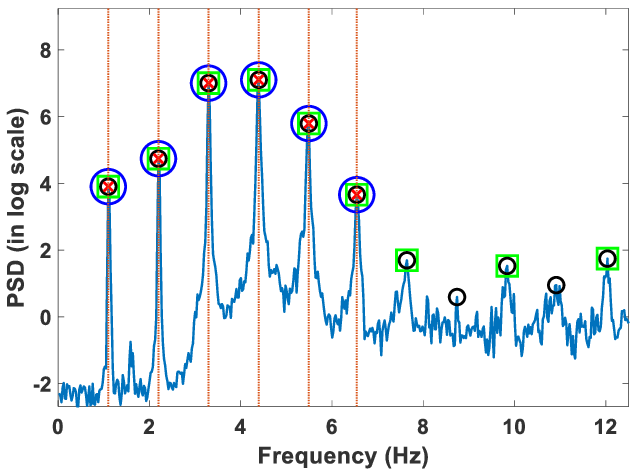
\includegraphics[width = 0.7\textwidth]{imagenes/cap1_marcoteo/peakpicking.png}
        \caption{Método de \textit{peak picking} \citep{peakpicking2021}.}
        \label{fig:peakpicking}
    \end{figure}
    
    \item Estimación del amortiguamiento por ancho de banda local: Una vez identificadas las frecuencias naturales del sistema, es de interés conocer el factor de amortiguamiento que corresponde a cada uno. Para esto, se suele aplicar el método de ancho de banda local, también conocido como método de la potencia mitad. Consiste en estudiar el espectro de potencia y ubicar los valores en los cuales la potencia de la señal se reduce a la mitad, en el caso de la figura \ref{fig:potenciamitad}, estas frecuencias serían $f_{max}$ y $f_{min}$, siendo la diferencia entre ambos $\Delta f$ y la frecuencia central $f_o$. Una vez obtenidas estas frecuencias se calcula el amortiguamiento de la siguiente forma:
    
    \begin{equation}
        \%\zeta = \frac{\Delta f}{2f_o}
    \end{equation}
    
    \begin{figure}[H]
        \centering
        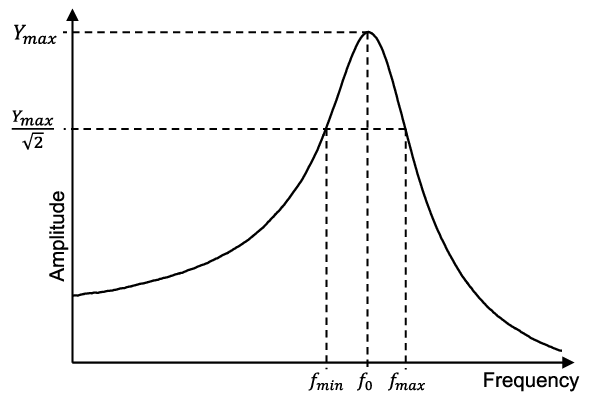
\includegraphics[width = 0.7\textwidth]{imagenes/cap1_marcoteo/Half-power-bandwidth-method.png}
        \caption{Método de obtención de amortiguamiento por ancho de banda local \citep{potenciamitad2019}.}
        \label{fig:potenciamitad}
    \end{figure}
\end{itemize}

% \subsection{Filtros Digitales}

\subsection{Aventanamiento}
\label{sec:aventanamiento}
Las señales provenientes de los sensores representan una ventana finita de tiempo, es decir, contienen una cantidad finita de datos. Es bien conocido que la FFT asume señales periódicas en el tiempo, eso se traduce en que las ecuaciones asumen que los datos se repiten una vez se termina el registro hasta el infinito. Esto genera discontinuidades notables en los bordes del registro que suelen verse como componentes frecuenciales que aparecen alrededor de las frecuencias naturales reales del sistema en estudio, fenómeno conocido como filtración de espectro o \textit{spectral leakage}, estas señales de alta frecuencia aparecen como ``\textit{alias}'' en las componentes de baja frecuencia, comportamiento que es indeseado para términos de análisis.

Para evitar este fenómeno se utiliza el método de aventanamiento, en el cual se multiplica la ventana de tiempo por una función que suaviza los ejes y disminuye su contribución en el espectro. Estas funciones hacen que los bordes del registro se ``encuentren'' como si se tratase de una señal periódica, resultando en un espectro mucho más limpio y en picos más claros.

Algunas de las funciones de aventanamiento más utilizadas:
\begin{itemize}
    \item Hanning.
    \item Hamming.
    \item Blackman.
\end{itemize}

\begin{figure}[H]
    \centering
    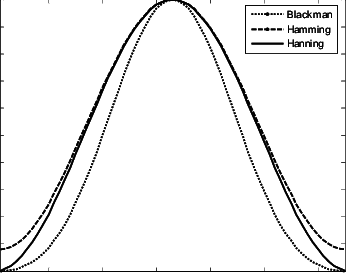
\includegraphics[width=0.6\textwidth]{imagenes/cap1_marcoteo/windows.png}
    \caption{Funciones de aventanamiento más utilizadas \citep{windowing2006}.}
    \label{fig:ventanas}
\end{figure}